\bluepage{Per fragment operace}

\begin{frame}[fragile]
\frametitle{Per fragment operace}
  \begin{itemize}
  \item Po fragment shaderu jsou na fragmenty aplikovány Per fragment operace
  \item Nejzákladnější operací je řešení viditelnosti pomocí depth testu
  \item Viditelnost se v OpenGL řeší pomocí Depth Buffer (paměť hloubky)
  \item Další testy jsou Stencil test a Scissor test
  \item Mezi jiné operace patří Blending, který se využívá pro průhledné objekty
  \end{itemize}
\end{frame}


\begin{frame}[fragile]
\frametitle{Depth Test a Depth Buffer}
  \begin{itemize}
  \item Depth test řeší viditelnost pomocí Depth Bufferu a to na úrovni fragmentů
  \item Různé způsoby nastavení
  \item Přesnost depth bufferu není nekonečná (většinou 24 bitů)
  \item Častý problem depth bufferu je jev známý jako depth Fight
  \item Brzký depth test - depth test může předběhnout vykonávání fragment shaderu
  \item Brzký depth test se provádí tehdy, pokud se ve fragment shaderu nemodifikuje hloubka fragmetu
  \item Brzký depth test může značně urychlit kreslení
  \end{itemize}
  {\scriptsize
  \begin{minted}[frame=lines]{c++}
glEnable(GL_DEPTH_TEST);//zapneme depth test - nastavi se stav pipeline
glDepthFunc(GL_LEQUAL);//fragment s mensi nebo stejnou hloubkou projde
glDepthMask(GL_TRUE);//maskovani zapisu do depth bufferu
  \end{minted}
  }
\end{frame}

\begin{frame}[fragile]
\frametitle{Bleding - průhledné objekty}
  \begin{itemize}
  \item Blending umožňuje kombinovat novou barvu s již zapsanou barvou ve framebufferu
  \item Blending je řízen pomocí blendovací operace, source a destination faktorů
  \item Blendovací operace jsou sčítání, odčítání, min, max, ...
  \item Source faktor se aplikuje na barvu fragmentu
  \item Destination faktor se aplikuje na barvu již uloženou ve framebufferu
  \item Nutnost kreslit ve správném pořadí
  \end{itemize}
  \begin{figure}[h]
  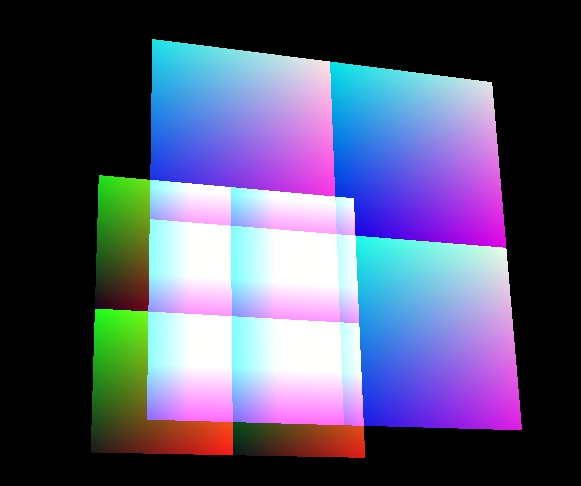
\includegraphics[width=3cm,keepaspectratio]{pics/blending.jpg}
  \end{figure}
  {\scriptsize
  \begin{minted}[frame=lines]{c++}
glEnable(GL_BLEND);//zapneme blending
glBlendEquation(GL_FUNC_ADD);//barvy se budou scitat
glBlendFunc(GL_SRC_ALPHA,GL_ONE_MINUS_SRC_ALPHA);//nastavime zpusob michani
  \end{minted}
  }
\end{frame}

